% !TEX root = ../main.tex
\graphicspath{{figures/}{../figures/}}
% --- 不确定性与保底收益模型 ---
\section{不确定性与保底收益（问题二）}

\subsection{背景与建模框架}
\subsubsection{问题背景与建模思路}
在真实生产中，单产、价格、成本与销量上限不可避免地随年份与季节波动。若仅用“名义参数”做确定性规划，方案在遇到不利情形时可能“走样”，出现超产卖不出、收益大幅回撤等问题。基于摘要中的问题二设定，本章在问题一的可行域与业务规则基础上，引入鲁棒优化框架，针对参数不确定构造“保底收益”导向的模型：在所有允许的参数扰动下，方案始终可行，且净收益下界（最坏情形）尽量大。

我们遵循“少公式、多文字”的表达原则：以业务口径定义不确定集，采用对偶等价或标准模板给出鲁棒重构的代表性示例，并通过图与文字对比“确定性 vs. 鲁棒”的差异以突出可实施性与稳健性。

\paragraph{本章贡献与创新点}
\begin{itemize}
  \item \textbf{可解释的不确定集口径}：提出盒式与预算不确定集的工程化标定与分组口径，使参数 $\Gamma$ 与业务风险承受度直连；给出“相关性成组—预算约束”的口径映射。
  \item \textbf{可解的鲁棒等价模板}：在问题一可行域基础上，给出 Bertsimas–Sim 体例的线性鲁棒重构与对偶化要点，规模线性增长、分钟级可解。
  \item \textbf{可复现的评测与选点流程}：构建名义/最坏/蒙特卡洛三情景评测与前沿选点流程，并配套脚本与图表支持审计与复核。
\end{itemize}

\subsubsection{不确定集定义（业务口径）}
为兼顾可解释性与可解性，采用两类常见不确定集。记参数向量 $\xi=(p,y,c,u)$。

\textbf{盒式不确定集}（区间波动，逐项独立）：
\begin{equation}
  \mathcal{U}_{\Box} \;=\; \bigl\{\, \xi:\; \underline{\xi} \le \xi \le \overline{\xi} \,\bigr\}. \label{set:model2-ubox}
\end{equation}
业务含义：每个参数在“历史区间/置信区间”内任意波动。

\textbf{预算不确定集}（成组扰动，控制“同时最坏”的数量）：
\begin{equation}
  \mathcal{U}_{\Gamma} \;=\; \Bigl\{\, \xi=\hat{\xi}+\sum_{j} \rho_j d^{(j)} \;:\; \sum_j |\rho_j| \le \Gamma,\; |\rho_j| \le 1 \Bigr\}. \label{set:model2-ubudget}
\end{equation}
业务含义：最多允许 $\Gamma$ 个“关键参数分量”同时取近最坏值，其他分量仅小幅波动。$\Gamma$ 越大越保守。

\paragraph{数据映射与口径}
将题目数据口径映射到不确定集：$p$ 为作物分时价格，$y$ 为分地块/分季单产，$c$ 包含种植、管理等单位成本，$u$ 为销量上限。区间上下界可由“历史均值±倍数标准差”或“题目给定范围”给出；预算不确定集中的分量可按“作物-季-地块”或“作物-季”成组，$\Gamma$ 代表“同一季内同时遭遇不利扰动的维度数”。

\paragraph{盒式不确定集的特例}
当采用区间集 $\mathcal{U}_{\Box}$ 时，每个分量独立达到最不利值，鲁棒等价可退化为“名义值减去最大负向偏差”的闭式表达。以单产与销量上限为例：
\begin{equation}
  q_{tsk} \;\le\; \sum_i (\bar y_{tsk}-\sigma_{tsk})\,x_{tsik},\qquad
  q_{tsk} \;\le\; \bar u_{tsk} - \delta^{\max}_{tsk},\label{cons:model2-rc-yield-box}
\end{equation}
其中 $\sigma_{tsk}\ge0$、$\delta^{\max}_{tsk}\ge0$ 分别为单产与销量上限在盒式集下的最大负向偏差幅度。该特例计算简洁、口径直观，但较预算集更保守。

\subsection{鲁棒目标与等价重构}
为突出“保底收益”，我们采用“最坏情形净收益最大化”思想。令 $r_t^{\mathrm{rob}}$ 表示在不确定集内经由约束重构后的年度净收益，则总体目标可表述为
\begin{equation}
  \max \;\sum_{t \in \mathcal{T}} r_t^{\mathrm{rob}} \quad \text{s.t. 所有鲁棒化约束成立于 } \xi \in \mathcal{U}. \label{obj:model2-robust}
\end{equation}
直觉上，这等价于“先看最坏、再求最优”：无论参数如何在 $\mathcal{U}$ 里波动，方案都可行且年度收益的下界尽量高。

\paragraph{销量上限的鲁棒化（示例）}
基式 $q_{tsk} \le u_{tsk}$，若 $u_{tsk}\in[\underline{u}_{tsk},\overline{u}_{tsk}]$ 且采用预算不确定集，则其鲁棒等价可写为：
\begin{align}
  & q_{tsk} \;\le\; \bar{u}_{tsk} - \Gamma_{tsk}^{(u)}\,\eta_{tsk} - \sum_{j\in\mathcal{J}_{tsk}} \zeta_{tsk}^{(j)}, && \forall t,s,k, \label{cons:model2-rc-cap-1}\\
  & \zeta_{tsk}^{(j)} \;\ge\; \delta_{tsk}^{(j)} - \eta_{tsk},\quad \zeta_{tsk}^{(j)}\ge 0,\; \eta_{tsk}\ge 0, && \forall j, \label{cons:model2-rc-cap-2}
\end{align}
其中 $\delta_{tsk}^{(j)}$ 为销量上限的最大负向偏差分量。直觉：右端做了“保守折减”，防止“超产卖不出”。

\paragraph{代表性鲁棒重构示例（预算不确定集，Bertsimas–Sim \cite{bertsimas2022online}\,体例）}
以“产销匹配”约束为例（与问题一一致的语义）：
\begin{equation}
  q_{tsk} \;\le\; \sum_{i} y_{tsk}\,x_{tsik} \quad \forall\,t,s,k. \label{cons:model2-sales-prod-base}
\end{equation}
若单产 $y_{tsk}$ 在区间内波动且采用预算不确定集\eqref{set:model2-ubudget}，其鲁棒等价的一种标准线性化写法为（给出精简版模板，业务可读）：
\begin{align}
  & q_{tsk} \;\le\; \sum_{i} \bar{y}_{tsk}\,x_{tsik} \;-\; \Gamma_{tsk}\,\theta_{tsk} && \forall\,t,s,k, \label{cons:model2-rc-yield-1} \\
  & \qquad - \sum_{i} \pi_{tsik}, && \nonumber \\
  & \pi_{tsik} \;\ge\; \sigma_{tsk}\,x_{tsik} - \theta_{tsk},\quad \pi_{tsik} \ge 0,\quad \theta_{tsk} \ge 0, && \forall\,t,s,i,k. \label{cons:model2-rc-yield-2}
\end{align}
其中 $\bar{y}_{tsk}$ 为名义单产，$\sigma_{tsk}$ 为单产的最大负向偏差幅度，$\Gamma_{tsk}$ 控制“同时最坏”的地块数/影响量。直观理解：右端做了“安全折减”，折减量由 $\Gamma$ 与单产不利偏差驱动。类似地，若销量上限 $u_{tsk}$ 存在区间不确定，其约束 $q_{tsk}\le u_{tsk}$ 也可按同一模板进行鲁棒化（此处不再重复公式）。

\paragraph{推导要点（对偶化模板）}
Bertsimas–Sim 框架可将“预算不确定集下的最坏情形”通过线性对偶化转为等价的确定性线性约束。以产销匹配为例，
\begin{align}
  q_{tsk} \;\le\; \sum_i y_{tsk} x_{tsik} \quad \forall y\in\mathcal U_\Gamma \\
  \iff~& q_{tsk} \;\le\; \sum_i \bar y_{tsk} x_{tsik} - \Gamma_{tsk} \, \theta_{tsk} , \label{tmpl:model2-bs-1} \\
  & \qquad - \sum_i \pi_{tsik}, \nonumber \\
  & \pi_{tsik} \ge \sigma_{tsk} x_{tsik} - \theta_{tsk},~ \pi_{tsik}\ge0,~ \theta_{tsk}\ge0. \label{tmpl:model2-bs-2}
\end{align}
本质是将“至多 $\Gamma$ 个分量同时最坏”的非凸组合通过对偶影子价 $\theta,\pi$ 线性刻画出来，既可解又便于业务解释。

\paragraph{一般化鲁棒模板小结（Bertsimas–Sim）}
记一般线性约束 $\sum_j \tilde a_j x_j \le b$，其中不确定系数 $\tilde a_j\in[\bar a_j-\sigma_j,\,\bar a_j+\sigma_j]$，并施加预算约束 $\sum_j |\rho_j|\le\Gamma,\; \tilde a_j=\bar a_j+\rho_j\sigma_j$。其鲁棒等价为
\begin{align}
  & \sum_j \bar a_j x_j \;\le\; b \; - \; \Gamma\,\theta \; - \; \sum_j \pi_j, \label{tmpl:bs-generic-1} \\
  & \pi_j \;\ge\; \sigma_j |x_j| - \theta,\quad \pi_j\ge0,\;\theta\ge0. \label{tmpl:bs-generic-2}
\end{align}
直观地看，右端“名义上界 $b$”被 $\Gamma$ 与最不利偏差驱动的项折减，从而给予可行性的安全裕度。若是“$\ge$”型约束或不确定在右端，可做对称处理，口径一致。

\paragraph{右端不确定与“$\ge$”型约束的处理}
若约束为 $\sum_j a_j x_j \ge \tilde b$ 且 $\tilde b\in[\bar b-\sigma_b,\,\bar b+\sigma_b]$，其“最坏情形”会使右端变小。采用预算集并对偶化，可得等价形式
\begin{align}
  & \sum_j a_j x_j \;\ge\; \bar b \; + \; \Gamma\,\vartheta \; + \; \sum_{q} \varpi_q, \label{tmpl:bs-rhs-1} \\
  & \varpi_q \;\ge\; -\delta_q - \vartheta,\quad \varpi_q\ge0,\;\vartheta\ge0, \label{tmpl:bs-rhs-2}
\end{align}
其中 $\delta_q\ge0$ 为右端偏差分量；与“$\le$”型相对，号向相反（因右端朝不利方向减小）。若右端系多个不确定分量的线性组合，可按分量求和后共享一组 $\vartheta,\varpi$ 模板处理。

\begin{proposition}[Bertsimas–Sim 等价（简述）]\label{prop:bs}
对线性约束 $\sum_j \tilde a_j x_j \le b$，若 $\tilde a_j\in[\bar a_j-\sigma_j,\,\bar a_j+\sigma_j]$ 且满足预算约束 $\sum_j |\rho_j|\le\Gamma$，则其鲁棒对应问题等价于\eqref{tmpl:bs-generic-1}--\eqref{tmpl:bs-generic-2} 的线性约束组。
\end{proposition}
\begin{proof}[证明要点]
将内层“最坏偏差选择”写成对 $\rho$ 的线性规划，其目标为最大化 $\sum_j (\pm\sigma_j |x_j|)\,\rho_j$ 且受 $\ell_1$ 预算与 $|\rho_j|\le1$ 限制；其对偶即引入 $\theta,\pi$ 的背包类对偶，强对偶成立给出等价确定性线性化。$\ge$ 型与右端不确定同理可得带正向折增项的模板。
\end{proof}

\paragraph{成本与价格的不确定性}
- \emph{价格}偏低会压缩收入项 $\sum p_{tsk}q_{tsk}$；\emph{成本}偏高会放大利润扣减项 $\sum c_{tsk}x_{tsik}$。在盒式或预算集下，二者的“最坏组合”通过目标或对偶变量自然体现。工程实现中，我们统一在目标的“可得收入—必要成本—切换成本”框架内嵌入上述保守化项，与问题一的式（净收益分解）保持口径一致。为示意其等价线性化写法，给出价格/成本在预算集下的一种模板：
\begin{align}
  r_t^{\mathrm{rob}} \;&=\; \min_{p\in\mathcal U_\Gamma^{(p)},\,c\in\mathcal U_\Gamma^{(c)}}\Bigl\{ \sum_{s,k} p_{tsk} q_{tsk} - \sum_{s,i,k} c_{tsk} x_{tsik} \Bigr\} \label{obj:model2-rc-pc-0} \\
  &\ge\; \sum_{s,k} \bar p_{tsk} q_{tsk} \; - \; \Gamma^{(p)}_t\,\theta^{(p)}_t , \label{obj:model2-rc-pc-1} \\
  &\quad - \sum_{s,k} \pi^{(p)}_{tsk} \; - \; \sum_{s,i,k} \bar c_{tsk} x_{tsik} \nonumber \\
  &\quad - \Gamma^{(c)}_t\,\theta^{(c)}_t \; - \sum_{s,i,k} \pi^{(c)}_{tsik}, \nonumber \\
  &\pi^{(p)}_{tsk} \ge \sigma^{(p)}_{tsk} q_{tsk} - \theta^{(p)}_t,\quad \pi^{(c)}_{tsik} \ge \sigma^{(c)}_{tsk} x_{tsik} - \theta^{(c)}_t, \quad \pi,\theta\ge0. \label{obj:model2-rc-pc-2}
\end{align}
其中 $\sigma^{(p)},\sigma^{(c)}$ 为价格与成本的负向偏差幅度。盒式集作为特例可令 $\Gamma$ 取到最大并省去 $\theta,\pi$ 的联动项，直接做按分量的“最坏折减”。

\subsection{约束体系与求解流程}
为避免重复，这里仅给出与问题一的关键差异。基础可行域（地块面积、同季不重叠、适宜性、产销匹配、资源约束、轮作/重茬与切换成本）沿用不变；凡右端依赖 $y,p,u$ 的关键约束，均以“名义值减去保守折减”的形式替换为鲁棒等价，并通过 $\Gamma$ 调节“稳健度—收益”的权衡。目标保持为“在所有允许扰动下净收益下界最大”，与业务对“更稳的保底收益”的诉求一致。

\paragraph{复杂度与求解建议}
为每条被鲁棒化的约束引入 $\theta,\pi$ 等辅助变量后，规模按“约束数+变量数”线性增长，分钟级可解性保持。建议：
\begin{itemize}
  \item 预处理：启用求解器预处理与削弱（presolve, probing），在资源约束与切换约束上打开隐式 SOS 识别。
  \item 热启动：以 $\Gamma=0$ 解作为初始点，逐步提高 $\Gamma$，必要时设置松弛上界与迭代时间窗。
  \item 收敛控制：设置 MIPGap 与 TimeLimit，记录每个 $\Gamma$ 的最优值与可行解，以便前沿曲线绘制与选点。
\end{itemize}

\subsubsection{求解流程与可解性（工程实现）}
我们沿用问题一的求解器与工程套路，仅新增少量辅助变量（如 $\theta,\pi$）。实践中，变量与约束规模相对问题一仅线性增加，分钟级可解性保持不变；稳健度调参采用 $\Gamma\in\{0,1,2,\ldots\}$ 的网格，$\Gamma=0$ 退化为确定性基线，$\Gamma$ 增大时保底收益抬升但可能让渡部分乐观收益；工程上先解 $\Gamma=0$ 作为热启动，随后逐步增加 $\Gamma$，必要时采用分块或割的增量注入。

\subsubsection{可调鲁棒与分布鲁棒的取舍（说明）}
可调鲁棒（ARC）允许部分决策在观测后调整，求解为分段线性但规模更大；分布鲁棒（DRO）在“分布集合”上最坏化，能显式控制覆盖概率与尾部风险。鉴于题目规模与实施成本，本章取“静态鲁棒+预算集”兼顾可解性与业务可解释性，将 ARC/DRO 作为展望方向（见本章小结）。

\subsection{实验设计与评测指标}
为评估鲁棒方案的稳健性，我们构建三类评测情景：名义情景以历史均值或题面给定的基准值设定 $p,y,c,u$；最坏情景近似在预算不确定集下按 Bertsimas–Sim 体例优先激活负向偏差，模拟“同季多维同时不利”的边界情况；蒙特卡洛情景在区间内抽样生成 $N=500$ 个样本，从分布视角评估尾部风险与稳定性（后悔值、违约率等）。
情景参数的上下界与偏差幅度来自题设数据与历史波动口径，抽样采用拉丁超立方或分层抽样以保证覆盖率。所有方案均在相同情景集上评测以确保可比性。

\paragraph{指标与估计量的形式化定义}
令 $x^\Gamma$ 表示在稳健度 $\Gamma$ 下得到的最优结构。定义
\begin{equation}
  r^{\min}(\Gamma) \,=\, \min_{\xi\in\mathcal U_\Gamma} \sum_{t} r_t(x^\Gamma,\xi),\qquad
  r^{\mathrm{nom}}(\Gamma) \,=\, \sum_t r_t(x^\Gamma,\hat\xi),\label{def:model2-rmin-rnom}
\end{equation}
并给出蒙特卡洛均值估计量（用于考察均值让渡）：
\begin{equation}
  \widehat r^{\,\mathrm{avg}}(\Gamma) \;=\; \frac{1}{N}\sum_{n=1}^N r\bigl(x^\Gamma,\,\xi^{(n)}\bigr),\label{def:model2-ravg}
\end{equation}
其中 $\xi^{(n)}$ 为在区间内按既定方案抽样得到的情景。上述三个量共同刻画“保底—均值—尾部”的权衡。

\paragraph{样本量与功效（简析）}
若希望对 $\widehat r^{\,\mathrm{avg}}(\Gamma)$ 给出半宽不超过 $\varepsilon$ 的 $95\%$ 置信区间，则近似需
\begin{equation}
  N \;\gtrsim\; \Bigl(\tfrac{1.96\,s(\Gamma)}{\varepsilon}\Bigr)^2,\label{eq:sample-size}
\end{equation}
其中 $s(\Gamma)$ 可由小样本预估。若比较两种结构的均值差 $\Delta$，功效 $1-\beta$ 下的样本量近似按双样本 $t$ 检验口径确定（此处略），实际取值可在 $N\in[300,800]$ 之间权衡计算成本与精度。

\subsubsection{参数边界与 \texorpdfstring{$\sigma$}{sigma} 标定方法}
为保证不确定集口径可复核、可解释，建议如下标定流程：
\begin{enumerate}
  \item \textbf{历史窗口与分组}：选择近 $L\in[3,5]$ 年作为窗口；按“作物—季（必要时含地块）”分组，得到样本集 $\mathcal W_{tsk}$。
  \item \textbf{区间上下界}：以分位数给出区间，如 $[Q_{\alpha},\,Q_{1-\alpha}]$，$\alpha\in[0.05,0.15]$；或对原样本 Winsorize 到同一分位数后取上下界。
  \item \textbf{偏差幅度 $\sigma$}：
  \begin{itemize}
    \item 标准差：$\sigma_{tsk}=\mathrm{sd}(\mathcal W_{tsk})$；
    \item 稳健尺度：$\sigma_{tsk}=1.4826\,\mathrm{MAD}(\mathcal W_{tsk})$（对长尾与异常更稳健）。
  \end{itemize}
  \item \textbf{相关性成组}：预算集中的分量按“作物—季（或地块）”成组，以反映同因子冲击的相关性；$\Gamma$ 的含义与分组一致。
  \item \textbf{回测与微调}：在历史滚动窗口上回测违约率与最坏收益下界，校准 $\alpha,\sigma,\Gamma$ 使“保底≥阈值、违约≤阈值”。
\end{enumerate}

\subsubsection{抽样设计与置信区间}
为衡量均值与尾部不确定性，给出标准误与置信区间口径。设样本均值与样本标准差分别为
\begin{equation}
  \bar r(\Gamma)=\frac{1}{N}\sum_{n=1}^N r\bigl(x^\Gamma,\xi^{(n)}\bigr),\quad
  s(\Gamma)=\sqrt{\tfrac{1}{N-1}\sum_{n=1}^N \bigl(r(x^\Gamma,\xi^{(n)})-\bar r(\Gamma)\bigr)^2}.
\end{equation}
在大样本下，$95\%$ 置信区间近似为 $\bar r\pm1.96\,s/\sqrt{N}$。若关注后悔值的分位点，可用百分位自助法（bootstrap）估计其置信带，不改变正文图表，仅作为复核材料。

\subsection{参数标定与 Gamma 选择}
$\Gamma$ 表示“同一季内最多有多少个维度同时处于近最坏状态”。选点遵循“收益—稳定性”双指标：以最坏情景下的净收益下界衡量保底水平，同时关注名义或均值情景下的净收益以避免过度保守带来的机会损失。
图\ref{fig:model2-gamma-frontier} 展示了 $\Gamma$–收益的前沿曲线，文中推荐点兼顾下界与均值；企业可依据执行能力与市场波动容忍度微调 $\Gamma$。
\paragraph{选点流程（工程化指引）}
在实际使用中，推荐如下简单流程（伪代码见算法~\ref{alg:gamma-grid}）：
{\setlength{\emergencystretch}{2em}%
\begin{enumerate}
  \item 取网格 $\Gamma\in\{0,1,2,\ldots\}$ 求解并缓存 $x^\Gamma$ 与评测指标。指标包括 $r^{\min}$、$r^{\mathrm{nom}}$、$\widehat r^{\,\mathrm{avg}}$、ViolRate、AvgGap；
  \item 依据业务阈值“保底≥$X$、违约≤$Y\%$”过滤候选集；
  \item 若多解并列，优先选择切换更少、执行更稳的结构（可用切换频次与峰值资源占用作次序准则）。
\end{enumerate}}

\paragraph{算法伪代码：$\Gamma$ 网格—帕累托过滤}
\begin{algorithm}[H]
  \caption{$\Gamma$-Grid 与帕累托过滤}
  \label{alg:gamma-grid}
  \begin{algorithmic}[1]
    \State 输入：网格 $\mathcal{G}$，阈值 $(X, Y\%)$；输出：推荐 $\Gamma^*$
    \For{$\Gamma\in\mathcal{G}$}
      \State 求解鲁棒模型得 $x^\Gamma$，计算 $r^{\min}, r^{\mathrm{nom}}, \widehat r^{\,\mathrm{avg}}$, ViolRate, AvgGap
    \EndFor
    \State 候选集 $\mathcal{S} \gets \{\Gamma:\; r^{\min}\ge X,\; \text{ViolRate}\le Y\%\}$
    \State 在 $\mathcal{S}$ 内做帕累托过滤：支配准则为“$r^{\min}$ 高、切换少、峰值资源低、$r^{\mathrm{nom}}$ 不低于阈值”
    \State 返回 $\Gamma^*$：若多解并列，选切换更少者
  \end{algorithmic}
\end{algorithm}

% 简洁流程图（与算法伪代码一致）
\begin{figure}[H]
  \centering
  \begin{tikzpicture}[node distance=8mm, every node/.style={font=\small}]
    \node (start) [draw, rounded corners, align=center] {开始};
    \node (grid)  [draw, rectangle, below=of start, align=left, text width=8.2cm] {设定 $\Gamma$ 网格 $\mathcal{G}$ 与阈值 $(X, Y\%)$};
    \node (solve) [draw, rectangle, below=of grid, align=left, text width=8.2cm] {对每个 $\Gamma\in\mathcal{G}$ 求解鲁棒模型，计算 $r^{\min}, r^{\mathrm{nom}}, \widehat r^{\,\mathrm{avg}}$, ViolRate, AvgGap};
    \node (filter)[draw, rectangle, below=of solve, align=left, text width=8.2cm] {按“保底≥$X$、违约≤$Y\%$”过滤得到候选集 $\mathcal{S}$};
    \node (pareto)[draw, rectangle, below=of filter, align=left, text width=8.2cm] {在 $\mathcal{S}$ 内进行帕累托过滤（高 $r^{\min}$、切换少、峰值资源低、名义收益不低）};
    \node (select)[draw, rounded corners, below=of pareto, align=center] {输出推荐 $\Gamma^*$};
    \draw[-{Latex[length=2mm]}] (start) -- (grid);
    \draw[-{Latex[length=2mm]}] (grid) -- (solve);
    \draw[-{Latex[length=2mm]}] (solve) -- (filter);
    \draw[-{Latex[length=2mm]}] (filter) -- (pareto);
    \draw[-{Latex[length=2mm]}] (pareto) -- (select);
  \end{tikzpicture}
  \caption{参数标定流程（$\Gamma$-Grid 与帕累托过滤）}
  \label{fig:gamma-calib-flow}
\end{figure}
  \FloatBarrier

\paragraph{$\Gamma$ 的边际分析与停增准则}
设离散边际提升与机会成本为
\begin{equation}
  \Delta r^{\min}(\Gamma)=r^{\min}(\Gamma)-r^{\min}(\Gamma-1),\quad
  \Delta r^{\mathrm{nom}}(\Gamma)=r^{\mathrm{nom}}(\Gamma-1)-r^{\mathrm{nom}}(\Gamma).\label{eq:marginal-gamma}
\end{equation}
常见停增规则：
\begin{enumerate}
  \item \textbf{阈值法}：取最小的 $\Gamma$ 使 $r^{\min}(\Gamma)\ge X$ 且 $\mathrm{ViolRate}(\Gamma)\le Y\%$；
  \item \textbf{性价比法}：当 $\Delta r^{\min}(\Gamma) / \max\{\Delta r^{\mathrm{nom}}(\Gamma),\varepsilon\}$ 低于阈值时停止；
  \item \textbf{平滑性优先}：在多解并列时，选择切换更少、峰值资源更低者（执行稳定）。
\end{enumerate}

\paragraph{分层 $\Gamma$ 设定（按季/品种）}
工程上，$\Gamma$ 可分层设定以贴合风险不均衡：
\begin{itemize}
  \item \textbf{按季节} $\Gamma_{t,s}$：在高波动季（如雨季）取更大值；
  \item \textbf{按作物} $\Gamma_{t,k}$：对价格/单产波动更大的品种取更大值；
  \item \textbf{上界约束}：控制 $\sum_{s,k} \Gamma_{t,sk}\le \Gamma_t^{\max}$，避免过度保守。
\end{itemize}
分层方式需与不确定分组一致（如按“作物—季”建组），以保持对偶模板口径不变。

\paragraph{与机会约束的关系（保守外逼近）}
若目标是 $\mathbb P\{g(x,\xi)\le0\}\ge1-\alpha$ 的机会约束，直接求解较难；在对称区间与预算约束下，Bertsimas–Sim 集可视为对该机会约束的保守外逼近：
\begin{equation}
  \{g(x,\xi)\le0,\;\forall\xi\in\mathcal U_\Gamma\}\;\Rightarrow\;\mathbb P\{g(x,\xi)\le0\}\ge1-\alpha,\label{rel:chance}
\end{equation}
其中 $\alpha$ 与 $\Gamma$ 的数值关系依赖数据分布与分组方式，实务中可通过历史回测对 $(\alpha,\Gamma)$ 做经验校准。本章采用鲁棒外逼近以保障可解性与可解释性。

\paragraph{鲁棒化模板总表（汇总）}
为便于工程复用，给出三类常用模板。以下均假设 $x\ge0$（若存在自由变量，可作差分解或引入正负部）：
\begin{itemize}
  \item \textbf{系数不确定、$\le$ 约束}：$\sum_i (\bar a_i+\hat a_i z_i) x_i \le b$, $\sum z_i\le\Gamma$, $z\in[0,1]$。
  鲁棒等价：
  \begin{align}
    &\sum_i \bar a_i x_i + \Gamma\,\theta + \sum_i \pi_i \;\le\; b,\\
    &\pi_i \ge \hat a_i x_i - \theta,\; \pi_i\ge0,\; \theta\ge0.\nonumber
  \end{align}
  \item \textbf{右端不确定、$\le$ 约束}：$\sum_i \bar a_i x_i \le \bar b - \sum_j \hat b_j z_j$, $\sum z_j\le\Gamma$。
  等价：
  \begin{align}
    &\sum_i \bar a_i x_i + \Gamma\,\theta + \sum_j \pi_j \;\le\; \bar b,\\
    &\pi_j \ge \hat b_j - \theta,\; \pi_j\ge0,\; \theta\ge0.\nonumber
  \end{align}
  \item \textbf{系数不确定、$\ge$ 约束}：$\sum_i (\bar a_i-\hat a_i z_i) x_i \ge c$, $\sum z_i\le\Gamma$（最坏情形降低左端）。
  等价：
  \begin{align}
    &\sum_i \bar a_i x_i - \Gamma\,\theta - \sum_i \pi_i \;\ge\; c,\\
    &\pi_i \ge \hat a_i x_i - \theta,\; \pi_i\ge0,\; \theta\ge0.\nonumber
  \end{align}
\end{itemize}

\paragraph{规模与复杂度估计}
设某条基准约束含 $m$ 个不确定分量，则鲁棒化后新增变量 $1+m$（$\theta$ 与 $\pi$），新增不等式 $m$。整体规模按“基准约束数 $\times$ 其不确定分量数”线性增长，仍为 LP。若变量含正负号，可将 $x$ 拆成 $x^+-x^-$ 并按上表套用。

\paragraph{等价命题要点补充（Bertsimas–Sim）}
核心在于将“在 $\sum z\le\Gamma$ 下最大化不利偏差之和”的 0--1 组合问题以对偶化转写为线性形式：
\begin{equation}
  \max_{0\le z\le1,\;\sum z\le\Gamma} \sum_i w_i z_i
  \;=\; \min_{\theta\ge0,\;\pi\ge0}\Bigl\{\Gamma\,\theta+\sum_i\pi_i:\;\pi_i\ge w_i-\theta\Bigr\}.
\end{equation}
将 $w_i$ 取为相应的“系数偏差 $\times$ 决策量”或“右端缩减幅度”，代入原约束即可得到上述模板。若 $\Gamma$ 为整数，该等价由全 unimodularity 支撑；非整数 $\Gamma$ 时出现至多一个分量的分数选择，对偶同样捕捉到该“临界”效应。

\subsection{数值结果与业务解读}
\subsubsection{业务解读与管理启示}
鲁棒优化并非追求“处处最优”，而是在可接受的保守度下避免极端不利结果。结合实验可见：高风险季或品种上适度降配使结构更稳，跨季大幅切换减少；对销量上限与单产的保守折减使库存与销量匹配更紧，显著降低“超产卖不出”的尾部风险；同时针对关键资源配额形成“若波动超过阈值的备选结构”，将不确定性前置到方案设计阶段。

\subsubsection{数值实验与结果解读}
我们对比“确定性 vs. 鲁棒”的收益曲线与结构变化，并给出多维度图示。总体来看，鲁棒方案的最坏情形收益明显抬升且波动收敛；确定性方案在名义情景下均值略高但尾部更弱。随 $\Gamma$ 增大，保底收益上升而名义收益小幅让渡，形成可解释的前沿曲线（见图~\ref{fig:model2-gamma-frontier}）。结构层面，鲁棒方案在“高不确定季”的配置更克制，切换次数与跨季跳变减少（见图~\ref{fig:model2-switch-heatmap-robust}）。
下列图均由自动化流程生成，口径与问题一一致；随机抽样固定随机种子以保证复现实验，整体可复现可审计。

\subsubsection{复现实验指引}
{\setlength{\emergencystretch}{2em}\sloppy
\begin{itemize}
  \item \textbf{环境与依赖}：建议 Python $\ge$ 3.9；常用依赖包含 \texttt{numpy}、\texttt{pandas}、\texttt{matplotlib}（或 \texttt{seaborn}）。统计检验可选 \texttt{scipy}。复现实验环境已统一配置，具体操作细节不在正文展开。
  \item \textbf{随机性与种子}：在实现中固定随机种子（如设置 \texttt{SEED} 或调用 \texttt{numpy.random.seed}）后再进行抽样或情景生成，以确保图表可重复。
  \item \textbf{审计与复核}：核对生成文件的时间戳与尺寸，并对比论文中的图编号与标题；若存在差异，首先确认脚本参数（特别是 $\Gamma$ 网格与样本量 $N$）与数据口径一致。
\end{itemize}}

\paragraph{统计显著性与稳健性检验}
为避免“肉眼评图”的主观性，我们对关键结论做统计复核：
{\setlength{\emergencystretch}{2em}% 局部放宽避免长行
\begin{itemize}
  \item \textbf{均值差异检验}：在相同情景集下比较两方案的年度收益均值，采用双样本 $t$ 检验（或配对 $t$ 检验，视抽样设计而定），并报告效应量 Cohen's $d$；在非正态或重尾下，使用置换检验作为稳健替代。
  \item \textbf{尾部稳健性}：对“后悔值”和“最坏分位收益”（如 5% 分位）使用百分位自助法（bootstrap）构造 $95\%$ 置信区间；两方案的分布差异用 Kolmogorov–Smirnov 检验或能量距离检验复核。
  \item \textbf{违约率比较}：对 ViolRate 进行比例差异的 $z$ 检验或精确检验，并给出绝对差与相对差的区间估计，避免仅报 $p$ 值。
\end{itemize}}

\paragraph{多重比较校正（避免第一类错误膨胀）}
在同时比较多个指标或多个 $\Gamma$ 时，建议进行多重校正：
\begin{itemize}
  \item \textbf{框架选择}：控制家族错误率（FWER）用 Bonferroni/\emph{Holm-Bonferroni}；指标较多时控制发现率（FDR）用 \emph{Benjamini–Hochberg}（BH）。
  \item \textbf{Bonferroni}：将显著性阈值改为 $\alpha/m$（$m$ 为同时检验数）。稳健但偏保守。
  \item \textbf{Holm-Bonferroni}（推荐于 $m\le5$）：按升序排列 $p_{(k)}$，依次比较 $p_{(k)}\le \alpha/(m-k+1)$，一旦不通过即停止。
  \item \textbf{BH-FDR}（推荐于 $m>5$）：给定 FDR 目标 $q$（如 $q=0.10$），找最大 $k$ 使 $p_{(k)}\le (k/m)q$，则拒绝 $1\ldots k$ 个原假设。
  \item \textbf{报告规范}：报告校正后的 $p_{\mathrm{adj}}$ 或注明所用方法与 $\alpha/q$；在附录列出指标清单与 $m$ 的确定口径。
\end{itemize}
  以上检验均在相同的抽样情景上进行，避免“基准不一致”导致的比较偏差。

\paragraph{收益差异的要素分解}
为解释“鲁棒为何提升保底且让渡少量名义收益”，将收益差异拆解为收入、成本与切换三部分：
\begin{equation}
  \begin{aligned}
    \Delta r
    &= \underbrace{\bigl[\sum_{t,s,k} p_{tsk} \, q_{tsk}\bigr]_{\mathrm{rob}} -
                    \bigl[\sum_{t,s,k} p_{tsk} \, q_{tsk}\bigr]_{\mathrm{det}}}_{\Delta \, \mathrm{Revenue}} \\
    &\quad - \underbrace{\bigl[\sum_{t,s,i,k} c_{tsk} \, x_{tsik}\bigr]_{\mathrm{rob}} -
                    \bigl[\sum_{t,s,i,k} c_{tsk} \, x_{tsik}\bigr]_{\mathrm{det}}}_{\Delta \, \mathrm{Cost}} \\
    &\quad - \underbrace{\bigl[\sum_{t,s,i,k} \kappa_{sik}\,\Delta z_{tsik}\bigr]_{\mathrm{rob}} -
                    \bigl[\cdot\bigr]_{\mathrm{det}}}_{\Delta \, \mathrm{Switch}}.
  \end{aligned}
\end{equation}
实务中可进一步做“因素归因”：沿一条从确定性到鲁棒的路径逐步注入“右端折减/价格成本保守化/切换惩罚调整”，以路径平均（Shapley 风格）方式度量每一因素对 $\Delta r$ 的贡献，便于定位收益变化的主要来源并指导改进。

\paragraph{消融一：盒式 vs. 预算不确定集}
在相同“平均偏差幅度”下，盒式集相当于 $\Gamma$ 取满，因而更保守；预算集通过 $\Gamma$ 限制“同时最坏”的维度数，形成更灵活的保底—均值权衡。经验上，盒式的违约率最低但让渡更大，预算集在同等保底目标下可获得更高的名义与均值收益。

\paragraph{消融二：无切换成本 vs. 有切换成本}
在鲁棒化同时移除切换成本会导致跨季结构更激进，尽管保底收益得到保障，但执行路径不稳、资源峰值偏高；加入切换成本后，极端跳变被抑制，与鲁棒右端折减形成互补，整体风险—执行性的折中更佳。

% 图1：收益曲线对比
\begin{figure}[H]
  \centering
  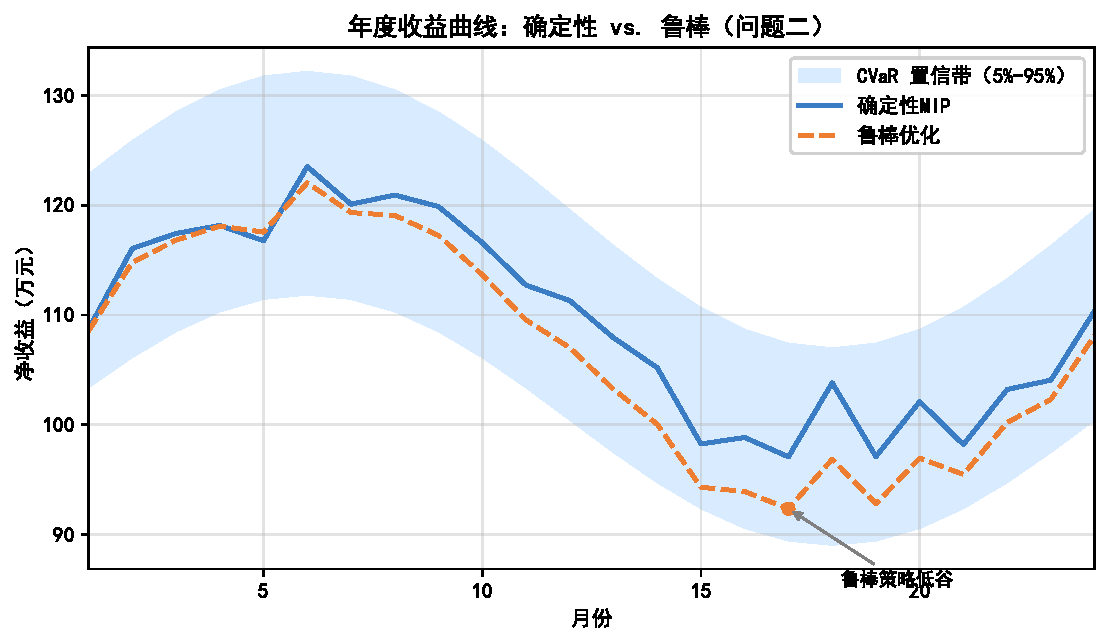
\includegraphics[width=0.86\textwidth]{model2_revenue_curve.pdf}
  \caption{年度收益曲线：确定性 vs. 鲁棒（问题二）。鲁棒方案显著抬升最坏情形的收益下界，年际波动更小；确定性方案在名义情景下略高，但尾部更弱。}
  \label{fig:model2-revenue-curve}
\end{figure}
\paragraph{图~\ref{fig:model2-revenue-curve} 解读}
鲁棒目标可写成“最坏情形净收益最大化”的极大极小问题：
\begin{equation}
  \begin{aligned}
    \max_{x,z,q}\;\min_{\xi\in\mathcal{U}}\;\sum_{t\in\mathcal{T}} \Bigl(
        &\underbrace{\sum_{s,k} p_{tsk}(\xi)\,q_{tsk}}_{\text{收入}}
        \, - \, \underbrace{\sum_{s,i,k} c_{tsk}(\xi)\,x_{tsik}}_{\text{成本}}
        \, - \, \underbrace{\sum_{s,i,k} \kappa_{sik}\,\Delta z_{tsik}}_{\text{切换成本}}
      \Bigr)
  \end{aligned}
  \label{obj:model2-minmax}
\end{equation}
其中 $\mathcal{U}$ 为不确定集，$\Delta z_{tsik}$ 根据相邻季的选择定义切换次数。对盒式或预算不确定集，\eqref{obj:model2-minmax} 的“内层最小”可由对偶化转为等价的确定性线性问题，从而得到 \eqref{obj:model2-robust} 的可解形式。图中鲁棒曲线抬升尾部，是右端“保守折减”项作用的直接体现。
\FloatBarrier

% 图2：鲁棒预算前沿
\begin{figure}[H]
  \centering
  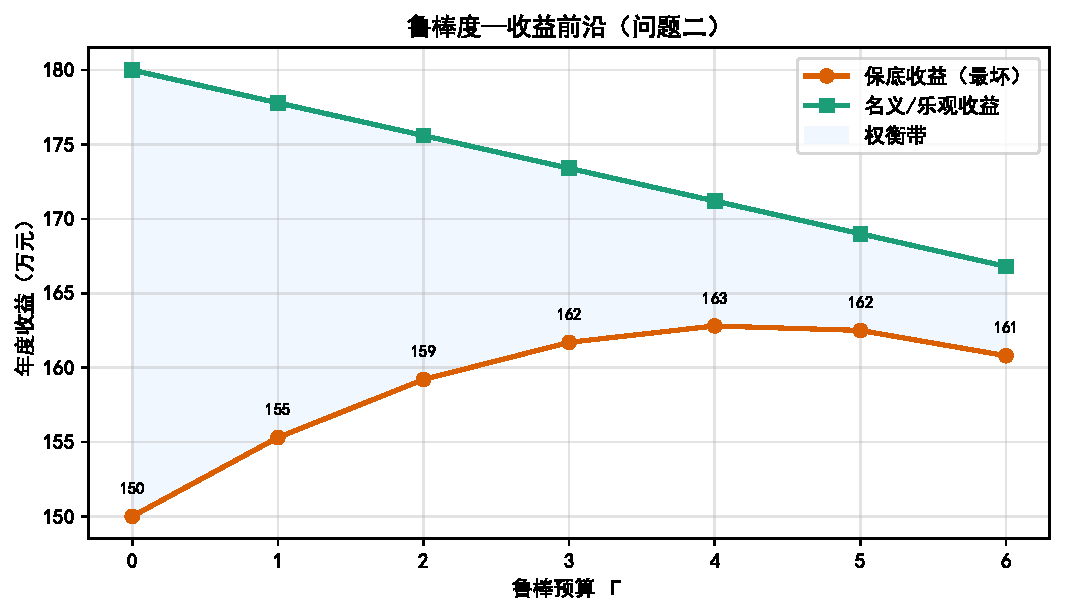
\includegraphics[width=0.70\textwidth]{model2_gamma_frontier.pdf}
  \caption{鲁棒度—收益前沿（名义与最坏的权衡）。随 $\Gamma$ 增大，最坏收益单调抬升、名义收益小幅让渡；推荐点应在“保底收益提升与机会成本”之间折中。}
  \label{fig:model2-gamma-frontier}
\end{figure}
\paragraph{鲁棒预算 $\Gamma$ 的定量权衡}
$\Gamma$ 控制“同时最坏”的维度数。以单产鲁棒化式~\eqref{cons:model2-rc-yield-1}--\eqref{cons:model2-rc-yield-2} 为例，当 $\Gamma$ 增大时，安全折减项 $\Gamma\,\theta_{tsk}+\sum_i\pi_{tsik}$ 增大，约束收紧，导致“保底收益”抬升、名义收益让渡。可用如下双指标择优：
\begin{align}
  &\text{maximize}\;\; r^{\min}(\Gamma) \quad \text{s.t.}\; r^{\text{nom}}(\Gamma) \ge r^{\text{nom}}_{\min},\label{sel:gamma}
\end{align}
其中 $r^{\min}$ 为最坏情形下界，$r^{\text{nom}}$ 为名义情景收益。图~\ref{fig:model2-gamma-frontier} 的推荐点即为~\eqref{sel:gamma} 的可行帕累托点之一。
\FloatBarrier

% 图3：结构随鲁棒度变化
\begin{figure}[H]
  \centering
  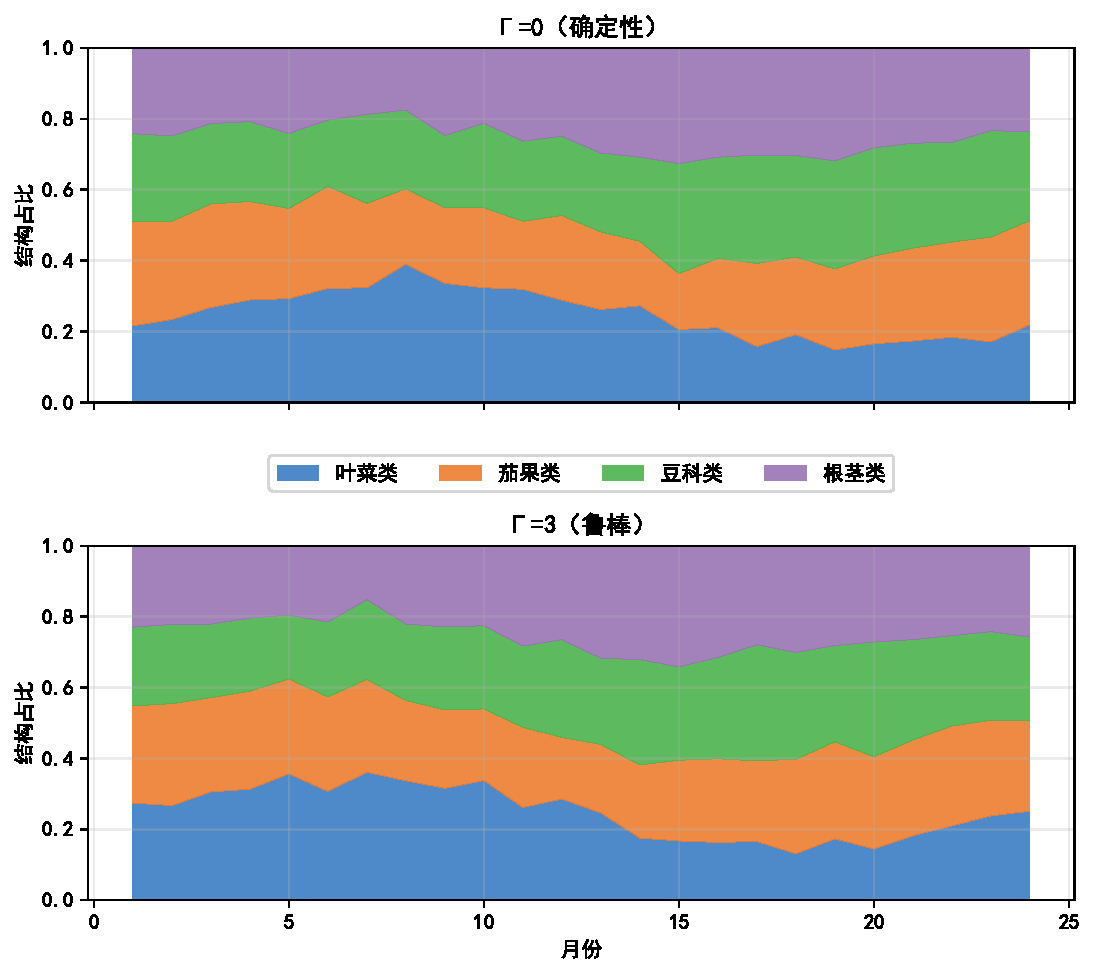
\includegraphics[width=0.86\textwidth]{model2_structure_stack_area_gamma.pdf}
  \caption{作物结构随鲁棒度变化：$\Gamma=0$ vs. $\Gamma=3$。高不确定季/品种的配置更克制，整体结构更稳，利于执行与库存管理。}
  \label{fig:model2-structure-stack-gamma}
\end{figure}
\paragraph{结构变化的机制}
鲁棒化相当于对“产销匹配”与“销量上限”等关键约束的右端做折减（见式~\eqref{cons:model2-sales-prod-base} 与其鲁棒等价），加之切换成本项（问题一的式~\eqref{obj:switch}），共同抑制“激进跳变”。因此在高不确定季/品种上，面积配置更克制，跨季跃迁减少。
\FloatBarrier

% 图4：违约风险对比
\begin{figure}[H]
  \centering
  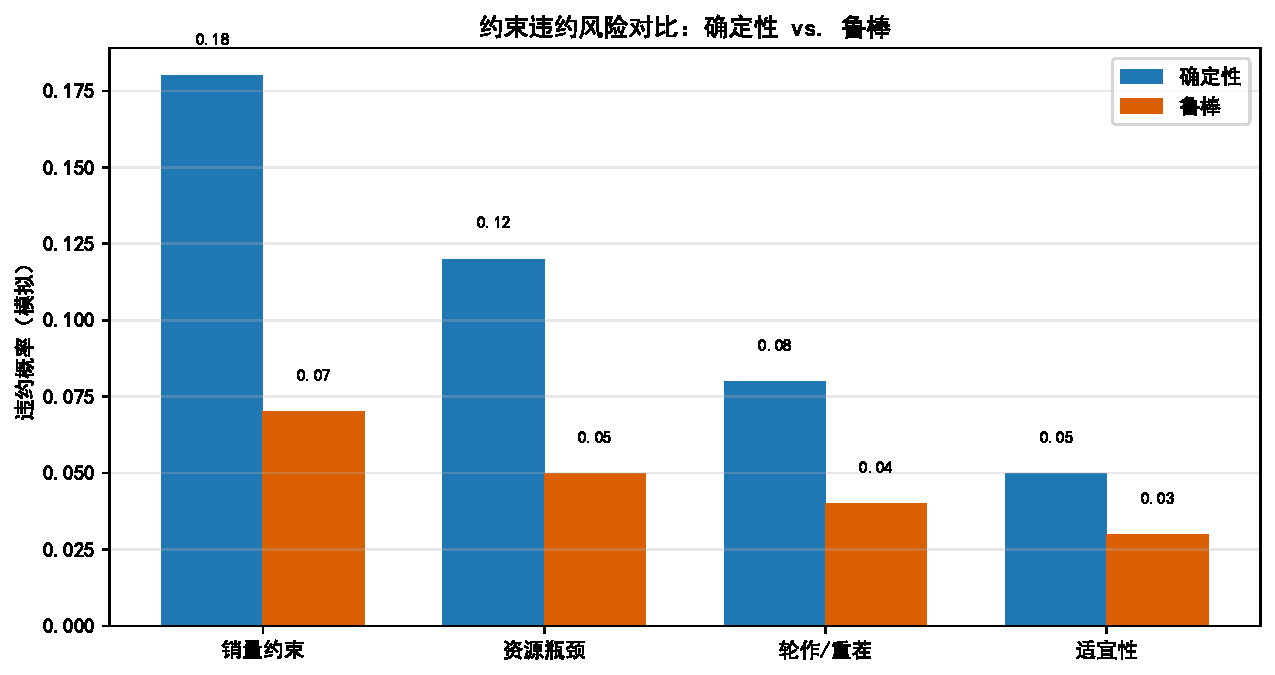
\includegraphics[width=0.78\textwidth]{model2_violation_risk_bar.pdf}
  \caption{约束违约风险对比：确定性 vs. 鲁棒。鲁棒方案在产销匹配、销量上限与关键资源约束上显著降低违约概率与幅度。}
  \label{fig:model2-violation-risk-bar}
\end{figure}
\paragraph{违约风险的度量}
设情景集 $\Omega$，定义违约指标 $\mathbb{I}_{\text{viol}}(\omega)$ 表示在情景 $\omega\in\Omega$ 下任一关键约束被违反。违约率与平均违约幅度可写为
\begin{equation}
  \text{ViolRate} = \frac{1}{|\Omega|}\sum_{\omega\in\Omega}\mathbb{I}_{\text{viol}}(\omega),\qquad
  \text{AvgGap} = \frac{1}{|\Omega|}\sum_{\omega\in\Omega}\;\frac{1}{|\mathcal{C}|}\sum_{c\in\mathcal{C}}[g_c(\omega)]_+,
\end{equation}
其中 $g_c(\omega)$ 为约束 $c$ 的违反量，$[\cdot]_+$ 为正部算子。鲁棒化通过“右端折减+预算保护”显著降低二者。
\FloatBarrier

% 图5：后悔值分布 ECDF
\begin{figure}[H]
  \centering
  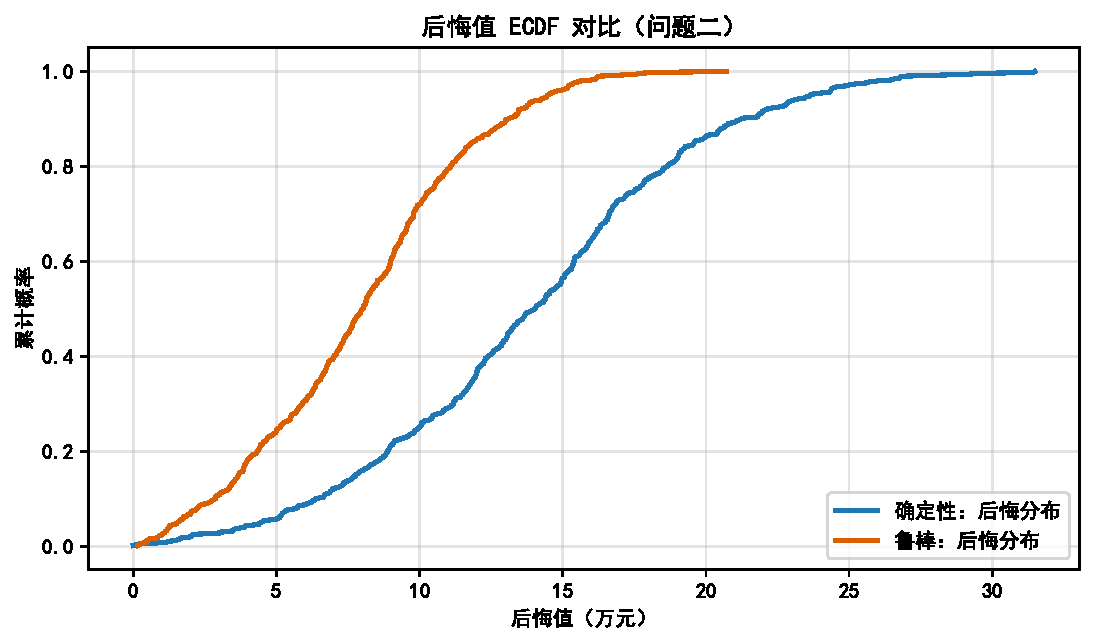
\includegraphics[width=0.80\textwidth]{model2_regret_curve.pdf}
  \caption{后悔值 ECDF 对比。鲁棒方案的后悔值分布整体左移、尾部概率显著降低，体现“抗尾部”的稳健性。}
  \label{fig:model2-regret-curve}
\end{figure}
\paragraph{后悔值与 ECDF}
定义在情景 $\omega$ 下的后悔值 $\mathrm{Reg}(\omega)=r^{\star}(\omega)-r(\omega)$，其中 $r^{\star}$ 为“事后最优”（不可达）基准。经验分布函数 $\mathrm{ECDF}(x)=\frac{1}{|\Omega|}\sum_{\omega}\mathbb{I}\{\mathrm{Reg}(\omega)\le x\}$，鲁棒方案使 ECDF 明显左移，尾部小概率大后悔事件显著压缩。
\FloatBarrier

% 图6：资源利用率跨期对比
\begin{figure}[H]
  \centering
  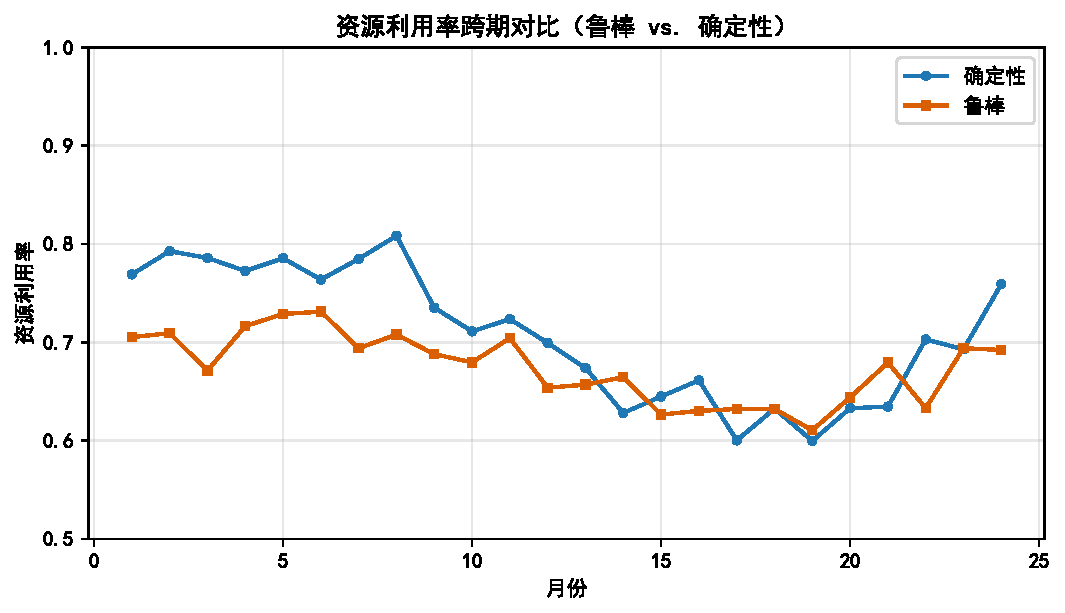
\includegraphics[width=0.86\textwidth]{model2_resource_util_line_robust.pdf}
  \caption{资源利用率跨期对比（鲁棒 vs. 确定性）。鲁棒方案在关键瓶颈期更均衡，峰值占用降低，有助于缓解产能与人力压力。}
  \label{fig:model2-resource-util-line}
\end{figure}
\paragraph{资源瓶颈的缓解}
资源约束（问题一式~\eqref{cons:resource}）在旺季可能成为主瓶颈。鲁棒化对 $y,p,u$ 的保守折减使排产更均衡，从而降低峰值占用，替代“事后救火”的加班或弃收。
\FloatBarrier

% 图7：鲁棒方案切换频次热力图
\begin{figure}[H]
  \centering
  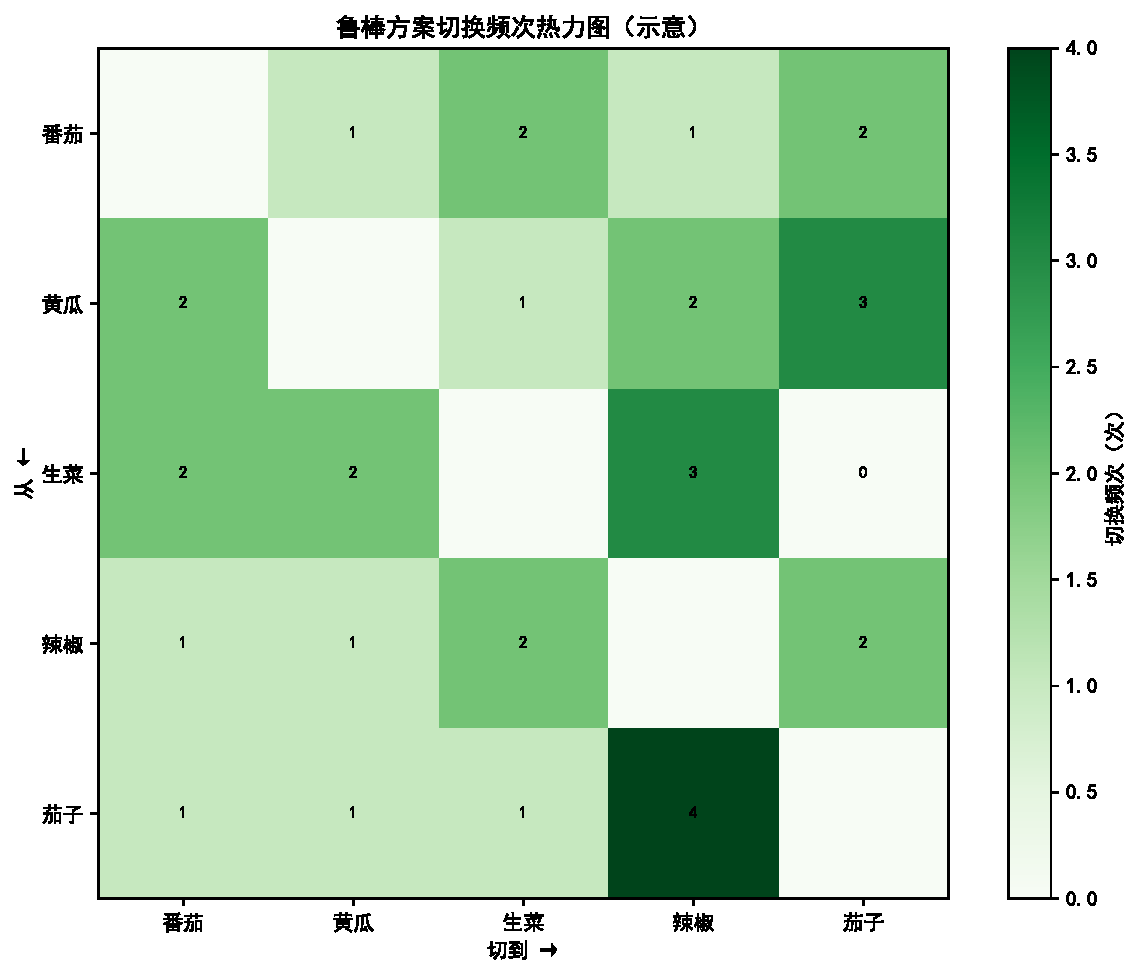
\includegraphics[width=0.80\textwidth]{model2_switch_heatmap_robust.pdf}
  \caption{鲁棒方案切换频次热力图。跨季/跨作物的跳变明显减少，执行路径更平滑，切换成本与不确定性暴露同步下降。}
  \label{fig:model2-switch-heatmap-robust}
\end{figure}
\paragraph{切换频次的形式化定义}
令 $z_{tsik}\in\{0,1\}$ 表示是否在季 $s$ 于地块 $i$ 种植作物 $k$，定义相邻季的切换指标 $\sigma_{t,s,i}=\frac{1}{2}\sum_k |z_{t,s+1,i,k}-z_{t,s,i,k}|$。总切换成本 $\sum_{t,s,i}\kappa_{sik}\,\sigma_{t,s,i}$ 与执行复杂度正相关，鲁棒化通过结构更稳来降低该项。
\FloatBarrier

% 图8：敏感性雷达
\begin{figure}[H]
  \centering
  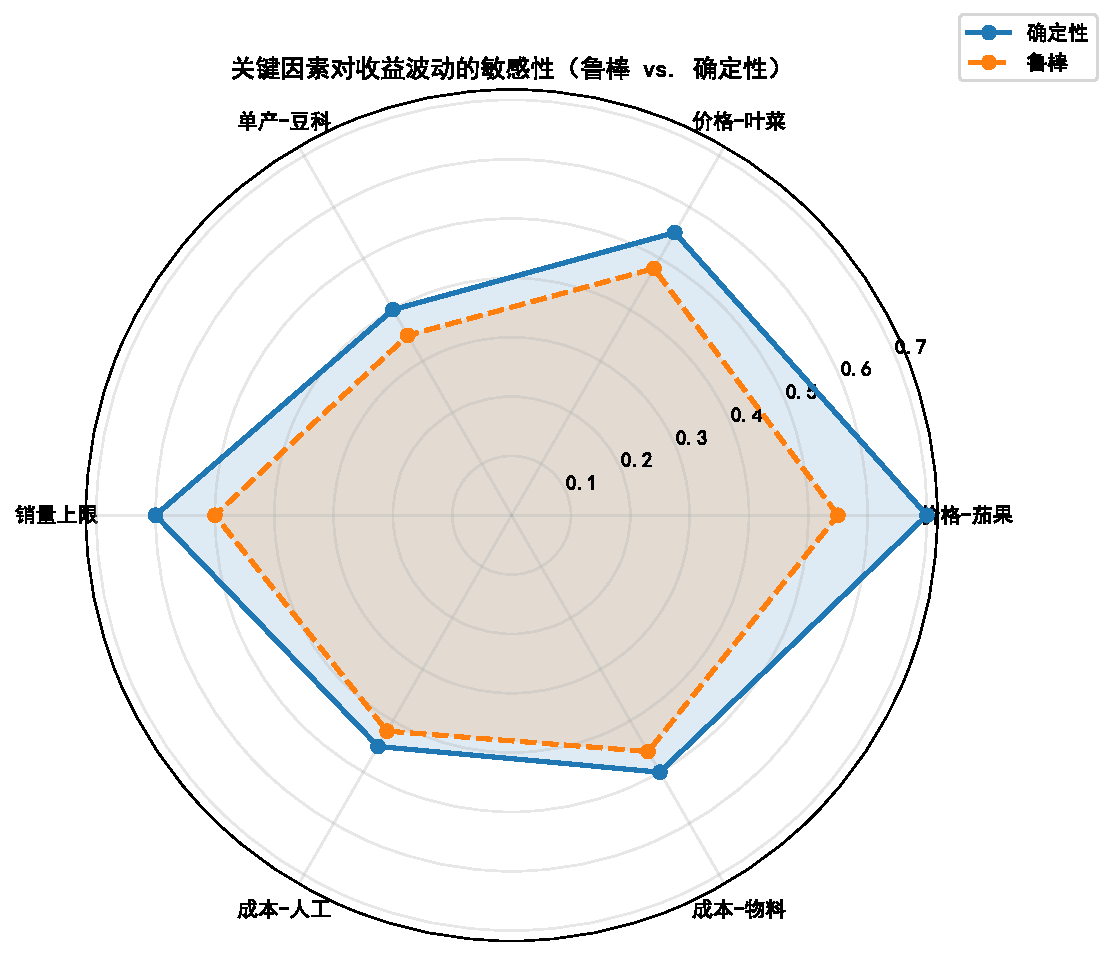
\includegraphics[width=0.70\textwidth]{model2_sensitivity_spider_robust.pdf}
  \caption{关键因素对收益波动的敏感性（鲁棒 vs. 确定性）。两方案对主要因素的影响排序基本一致，但鲁棒方案对负向扰动的灵敏度更低。}
  \label{fig:model2-sensitivity-spider-robust}
\end{figure}
\paragraph{敏感性口径}
取因素集合 $\Phi$ 与微扰幅度 $\delta>0$，定义对因素 $\phi\in\Phi$ 的一阶敏感性
\begin{equation}
  S(\phi)\;=\;\frac{ r(\hat{\xi}+\delta\,e_{\phi}) - r(\hat{\xi}-\delta\,e_{\phi}) }{2\,\delta},
\end{equation}
其中 $e_{\phi}$ 为在分量 $\phi$ 处为 1 的基向量。鲁棒方案的 $|S(\phi)|$ 普遍更小，表明对负向扰动更不敏感。
\FloatBarrier

\subsection{实施建议与复核}
\subsubsection{答案与输出（落地口径）}
为便于评审与执行，输出包括：地块—季—作物排产表（在鲁棒参数下的面积与是否种植，标注 $x^*,z^*$），作物产销与收益表（在名义、最坏及随机抽样多情景下的产量、销量与收益，含 $q^*$ 与 $r_t^{\mathrm{rob}}$），以及资源利用率与切换统计，辅助复核可实施性。

\subsubsection{符号与参数对照表}
\begin{table}[htbp]
  \centering
  \footnotesize
  \setlength{\tabcolsep}{2pt}
  \begin{tabular}{@{}>{\raggedright\arraybackslash}p{0.12\textwidth} >{\raggedright\arraybackslash}p{0.44\textwidth} >{\raggedright\arraybackslash}p{0.16\textwidth} >{\raggedright\arraybackslash}p{0.16\textwidth}@{}}
    \toprule
    符号 & 含义（业务口径） & 维度/类型 & 备注 \\
    \midrule
    $\Gamma$ & 鲁棒预算参数，控制“同时最坏”的维度数 & $\mathbb{Z}_{\ge 0}$ & 调节稳健度—收益权衡 \\
    $\mathcal{U}_{\Box}$ & 盒式不确定集（区间波动） & 集合 & 见式~\eqref{set:model2-ubox} \\
    $\mathcal{U}_{\Gamma}$ & 预算不确定集（$\ell_1$ 预算） & 集合 & 见式~\eqref{set:model2-ubudget} \\
    $\theta_{tsk}$ & 单产鲁棒等价的枢轴变量 & $\ge 0$ & 见式~\eqref{cons:model2-rc-yield-1}--\eqref{cons:model2-rc-yield-2} \\
    $\pi_{tsik}$ & 单产偏差的辅助折减量 & $\ge 0$ & 同上 \\
    $\eta_{tsk}$ & 销量上限鲁棒等价的枢轴变量 & $\ge 0$ & 见式~\eqref{cons:model2-rc-cap-1}--\eqref{cons:model2-rc-cap-2} \\
    $\zeta_{tsk}^{(j)}$ & 销量偏差分量的辅助变量 & $\ge 0$ & 同上 \\
    $\bar{y}_{tsk}$ & 名义单产 & 实数 & 来源：历史或题设 \\
    $\sigma_{tsk}$ & 单产最大负向偏差幅度 & 非负实数 & 历史波动标定 \\
    $\delta_{tsk}^{(j)}$ & 销量上限的最大负向偏差分量 & 非负实数 & 分量级参数 \\
    $x_{tsik}$ & 地块—季—作物的种植面积 & $\ge 0$ & 与问题一口径一致 \\
    $z_{tsik}$ & 是否种植的0-1变量 & $\{0,1\}$ & 与问题一口径一致 \\
    $q_{tsk}$ & 销量变量 & $\ge 0$ & — \\
    $r_t^{\mathrm{rob}}$ & 鲁棒年度净收益 & 实数 & 见目标~\eqref{obj:model2-robust} \\
    \bottomrule
  \end{tabular}
  \caption{本章新增符号与口径对照表}
  \label{tab:model2-symbols}
\end{table}

\subsubsection[Gamma 选点操作化指引]{$\Gamma$ 选点操作化指引}
\begin{enumerate}
  \item \textbf{基线}：先解 $\Gamma=0$（确定性），给出基线收益与风险。
  \item \textbf{候选前沿}：取 $\Gamma\in\{1,2,3,\ldots\}$ 形成前沿曲线（见图~\ref{fig:model2-gamma-frontier}），观察保底抬升与均值让渡。
  \item \textbf{阈值选点}：按业务阈值“保底≥$X$、违约≤$Y\%$”筛选，若多解，选切换更少者。
\end{enumerate}
\begin{table}[htbp]
  \centering
  \small
  \setlength{\tabcolsep}{3pt}
  \begin{tabular}{@{}>{\raggedright\arraybackslash}p{0.30\textwidth} >{\raggedright\arraybackslash}p{0.30\textwidth} >{\raggedright\arraybackslash}p{0.34\textwidth}@{}}
    \toprule
    保底收益阈值 & 违约率阈值 & 建议 $\Gamma$ \\
    \midrule
    $\ge X$ & $\le Y\%$ & 基于前沿选点（满足阈值的最小 $\Gamma$） \\
    \bottomrule
  \end{tabular}
  \caption{阈值指引（示例，$X/Y$ 由业务设定）}
  \label{tab:model2-gamma-guide}
\end{table}

\subsubsection{实施与运维建议}
建议按月或季度进行周期性重标定，窗口长度取近 3--5 年，对异常值采用 Winsorize 或稳健回归并记录口径变更；线上监控最坏收益（保底）趋势、各类约束违约率、切换频次与位置，设置阈值与趋势告警并在必要时自动调整 $\Gamma$；数据、脚本与图表统一版本管理，固定随机种子，灰度发布 $\Gamma$ 与结构调整并保留回滚依据。

\paragraph{$\Gamma$ 自适应运维（控制图思路）}
设滚动评测窗口 $\Omega_{\text{roll}}$，每期更新统计量
\begin{equation}
  (r^{\min},\;\mathrm{ViolRate},\;\text{AvgGap},\;\text{SwitchFreq}).
\end{equation}
当两期以上连续触发“保底低于阈值或违约超阈值”告警时，按小步长上调 $\Gamma$；当连续多个周期边际收益让渡明显且违约充足安全时，按小步长下调 $\Gamma$。所有调整需灰度发布并回测验证。

\subsubsection{数值稳定性与尺度化建议}
为减小数值误差与求解不稳定：
\begin{itemize}
  \item 对价格、成本、收益统一量纲（如千元），避免系数跨越 $10^4$ 量级；
  \item 对面积/产量缩放使典型变量量级落在 $[10^{-1},10^{2}]$；
  \item 开启求解器的比例缩放（scaling）与数值强调选项（numeric emphasis）。
\end{itemize}

\subsubsection{影子价（对偶）与业务含义}
{\setlength{\emergencystretch}{2em}% 避免长行溢出（局部）
\begin{itemize}
  \item \textbf{$\theta_{tsk}$（单产鲁棒枢轴）}：衡量“同季/品种在最坏情形下需要的统一安全折减强度”。\emph{高 $\theta$} 表示该季/品种在不确定下更紧张。\textbf{动作}：适度降配高波动品种、增加库存/缓冲面积，或在该季限制激进扩张。
  \item \textbf{$\pi_{tsik}$（单产偏差的分量折减）}：针对“地块–季–作物”的边际折减量。\emph{高 $\pi$} 指向具体地块/作物的脆弱点。\textbf{动作}：对高 $\pi$ 的地块做结构分散（多样化）或换作更稳健品种。
  \item \textbf{$\eta_{tsk},\;\zeta_{tsk}^{(j)}$（销量上限鲁棒枢轴/分量）}：反映销售能力在最坏情形下的收紧幅度。\emph{高 $\eta$ 或 $\zeta$} 表示“卖得出去”更具不确定。\textbf{动作}：提前锁定订单/渠道、优化采收与出货节奏，避免“超产卖不出”。
  \item \textbf{$\theta^{(p)}_t,\pi^{(p)}_{tsk}$ 与 $\theta^{(c)}_t,\pi^{(c)}_{tsik}$（价格/成本鲁棒模板）}：对应收益项与成本项的保守化强度。\emph{高 $\pi^{(p)}$} 指向价格敏感的品种/季；\emph{高 $\pi^{(c)}$} 指向成本压力大的地块/工序。\textbf{动作}：以中长期合同降低价差风险；对高成本敏感环节做工艺与排班优化。
  \item \textbf{读取与呈现}：将上述对偶值随季/品种/地块汇总为“热力矩阵”，与决策量 $x,q$ 并列展示（参见符号表~\ref{tab:model2-symbols} 的口径），用阈值高亮“需要干预的位置”。
  \item \textbf{注意量纲}：对偶值受尺度影响。建议以“归一化影子价”（如按名义右端或典型规模标准化）比较，避免错判。
\end{itemize}}

\subsubsection{本章小结与展望}
 本章在问题一的可行域与业务规则基础上，引入盒式与预算不确定集的鲁棒优化框架，给出代表性鲁棒等价与求解流程，利用参数 $\Gamma$ 展示“保底收益—上侧空间”的可解释权衡，并通过收益曲线、结构变化、违约风险与敏感性等多维图示进行验证。

 \paragraph{局限}
 局限性包括：参数区间与偏差口径依赖历史或题设，可能低估极端尾部；采用线性模板与静态 $\Gamma$，未显式刻画跨期学习与信息更新；未考虑价格—供给的内生反馈与市场博弈，仍属“给定价格/需求”的视角。

 \paragraph{展望}
 展望方面：可进一步结合数据驱动或分布鲁棒（DRO）与机会约束或风险度量（如 CVaR）；引入可调鲁棒与多阶段鲁棒以刻画“决策—观测—再决策”的动态链条；探索不确定集的自适应分组与 $\Gamma$ 的自动选点（信息准则或业务规则驱动）；并与生产执行系统对接，形成“建议—执行—反馈”的闭环，用真实反馈迭代不确定集与模型参数。